\section{点积与叉积的另一种解释——张量}
在物理学中,我们知道恒定力$\bb{F}$作用于位移$\bb{D}$做 $\bb{F}\cdot \bb{D}$个单位的功。与位移不同,力无法直接测量,只能测量其效果(弹簧的伸长、应变仪电阻的变化等),而且,力与位移具有不同的物理单位。这表明力——更准确地说,表示力的矢量与位移位于不同的向量空间中。如果力以磅为单位,位移以英尺为单位,那么我们在两个向量空间中任意设置单位$x$轴向箭头$\rr{OI}$分别表示一磅力和一英尺距离。现在想一想:你将如何以图形方式计算$\bb{F}\cdot \bb{D}$? 你可以首先使这两个向量空间的正$x$、$y$和$z$轴重合,然后,由于$\rr{OI}$是任意选择的,因此我们可以拉伸或收缩一个$\rr{OI}$直到与另一个重合。最后,$\bb{F}$在$\bb{D}$方向上的正交投影长度将以图形方式乘以$\left| \bb{D} \right|$,从而获得一个以英尺·磅为单位的量。

所有这些想象中的推搡是为了赋予$\bb{F}\cdot \bb{D}$一个几何意义,以便人们可以进行图形计算(这是一种古老的艺术,现在很少有人实践。)难道没有一种更简单的方式来看待事物,不仅不影响数字计算,还能更好地反映不同类型的物理对象?当然有:一个力$\bb{F}$可以被认为是一个线性函数的代表,它把任何矢量$\bb{D}$(位移)转换成一个实数(称为$\bb{F}$作用于$\bb{D}$的功)。

类似但更详细的考虑也适用于叉积。例如,假设力$\bb{F}$作用于位置为$\bb{x}$的点$P$,将围绕O点的扭矩表示为$\bb{x}\times \bb{F}$,这引出了将矢量变换成矢量的线性算子的概念。这样的算子被称为二阶张量。张量这个名字来自弹性理论,在弹性理论中,在一个负载的弹性体中,应力张量作用于与一点处体元的某个面垂直的单位矢量,并给出作用在该点的平面上的张力(即每单位面积的力)。参见练习1.20。其他重要的二阶张量包括刚体动力学中的惯性张量、弹性中的应变张量和流体动力学中的动量-通量张量。

\begin{figure}[htbp]
	\centering
	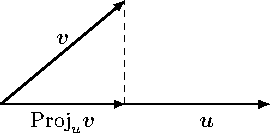
\includegraphics[width=0.4\textwidth]{./image/1.8.pdf}
	\caption{}
	\label{fig:1.8}
\end{figure}

我能想到的二阶张量的最简单且不平凡的例子如下。设向量$\bb{v}$在向量$\bb{u}$上的投影表示定义为
\begin{equation}\label{equ:1.27}
    \mathrm{Proj}_u\bb{v}=\left( \bb{v}\cdot \widehat{\bb{u}} \right) \widehat{\bb{u}}
\end{equation}

$\mathrm{Proj}_u\bb{v}$的几何含义如图\eqref{fig:1.8}所示。式\eqref{equ:1.27}的左边可以解释为算子$\mathrm{Proj}_u$作用于$\bb{v}$。式\eqref{equ:1.27} 的右边告诉我们算子$\mathrm{Proj}_u$将$\bb{v}$转换成一个$\bb{u}$方向上,大小为$\left| \bb{v}\cdot \widehat{\bb{u}} \right|$的矢量。为了符合标题中张量的要求,$\mathrm{Proj}_u$必须是线性的。但如果$\beta $和$\gamma $是任意标量,w是任意矢量,那么,根据点积的特性
\begin{align}
	\mathrm{Proj}_{\bb{u}}(\beta \bb{v}+\gamma \bb{w})&\equiv [(\beta \bb{v}+\gamma \bb{w})\cdot \widehat{\bb{u}}]\widehat{\bb{u}}\nonumber\\
	&=(\beta \bb{v}\cdot \widehat{\bb{u}}+\gamma \bb{w}\cdot \widehat{\bb{u}})\widehat{\bb{u}}\nonumber\\
	&=\beta (\bb{v}\cdot \widehat{\bb{u}})\widehat{\bb{u}}+\gamma (\bb{w}\cdot \widehat{\bb{u}})\widehat{\bb{u}}\nonumber\\
	&=\beta \mathrm{Proj}_{\bb{u}}\bb{v}+\gamma \mathrm{Proj}_{\bb{u}}\bb{w}\label{equ:1.28}
\end{align}
即$\mathrm{Proj}_u$是线性的,因此它是张量。现在做练习1.5以确保你可以在具体情况下应用这个张量。

式\eqref{equ:1.27}右边的形式反映了以下观点:两个向量$\bb{u}$和$\bb{v}$的直积$\bb{uv}$\footnote{许多作者也将直积$\bb{uv}$写作$\bb{u}\otimes \bb{v}$}是一个张量,它根据规则将任意一个向量$\bb{w}$转换成一个新的向量。
\begin{equation}\label{equ:1.29}
    \bb{uv}\left( \bb{w} \right) =\bb{u}\left( \bb{v}\cdot \bb{w} \right) 
\end{equation}
因此,特别地
\begin{equation}\label{equ:1.30}
    \mathrm{Proj}_{\bf{u}}=\widehat{\bb{u}}\widehat{\bb{u}}
\end{equation}

可以表示为直积的张量,如$\mathrm{Proj}_u$,被称为并矢。 正如我们马上要看到的,任何二阶张量都可以表示为并矢的线性组合。



